% \chapter{Demonstration of Utility}\label{ch:architecture}

% This chapter demonstrates how the reliability model introduced in \chref{ch:reliable-sots} can be realized in a concrete system implementation. The approach is illustrated through a running example implemented using a complex event processing (CEP) middleware architecture.

% Statecharts provide a formalism for specifying behavioural constraints using states, events, and transitions. Through this structure, they define the conditions under which system behaviours are permitted or restricted. When coupled to runtime logic, statecharts can be translated into executable controllers that influence how surrounding services operate during execution.

% In \chref{ch:reliable-sots}, statecharts were introduced to model lifecycle constraints governing the participation of constituents within a SoTS. By exposing lifecycle state through an executable state machine, external services can adapt their behaviour according to the current state of each constituent. In the implementation presented in this chapter, these statecharts supervise constituent participation within an event-driven processing pipeline, regulating how observations enter the CEP system and how compensation mechanisms respond to degraded behaviour.

% \section{Demonstration Using the Running Example}

% To demonstrate the practical utility of the reliability model, the running example introduced earlier is implemented using a CEP-based middleware architecture. The implementation realizes the Level~4 reliability configuration described in \chref{ch:reliable-sots}, combining lifecycle-based participation control with compensation mechanisms that reconstruct events when constituent data must be compensated for.

% In this system, multiple DTs produce event observations describing aspects of system activity. These observations represent measurements such as speed and engine temperature that are emitted as event streams. The observations are distributed through an event processing middleware and forwarded to a CEP engine that detects higher-level behaviours such as unsafe operating conditions.

% The lifecycle state of each constituent influences how observations are handled within the middleware. Depending on the participation state of a constituent, observations may be forwarded directly to the CEP pipeline, restricted, or reconstructed through compensation mechanisms. As constituents transition between lifecycle states, the corresponding state machines regulate how their observations are processed and how degraded behaviour is handled within the system.

% \subsection{Mapping the Architecture to Level-4 Reliability}

% The architecture operationalizes the Level~4 reliability configuration introduced in \chref{ch:reliable-sots}. Level~4 combines lifecycle-based participation control with adaptive compensation mechanisms to prevent degraded constituents from destabilizing system behaviour.

% Lifecycle constraints are enforced through executable statecharts that maintain the belonging and health state of each constituent. These statecharts regulate participation within the event processing pipeline by influencing how observations are emitted and processed based on the current lifecycle state.

% When constituent behaviour degrades, compensation services reconstruct events using state estimation techniques. This mechanism maintains a consistent event flow while allowing degraded constituents to operate in restricted roles or exit the system if necessary. Together, lifecycle control and compensation ensure that degraded constituents are progressively constrained while the CEP pipeline continues to operate using reliable observations.















\chapter{Demonstration of Utility}\label{ch:architecture}
% This is the entire point the chpater should get across and the relevancy of the information presented should always be relevant to this, if its not its too much info, we only need enough for the thesis level
This chapter demonstrates the practical utility of the reliability model introduced in Chapter X. The model is realized through an event-driven architecture in which lifecycle statecharts regulate constituent participation while compensation mechanisms address degraded observations. The chapter first presents the architectural design used to operationalize the model, then describes the implementation of the CEP-based middleware, and finally introduces the evaluation setup used to assess the impact of the proposed reliability mechanisms.



% need to explain the groudning scenario on what were building and then how maps like architectural mechanims to certain concepts in this, shoudl specifically 

% then this becomes a subsection where we explain the compnents that have now been justified above
% The architecture operationalizes Level-4 reliability through lifecycle-controlled event emission and compensation-based disturbance 










\chapter{Demonstration of Utility}\label{ch:architecture}

This chapter demonstrates the practical utility of the reliability model introduced in \chref{ch:reliable-sots}. The model is operationalized through an event-driven architecture in which executable lifecycle statecharts regulate constituent participation while compensation mechanisms mitigate disturbances affecting event observations.

The architecture serves as a proof-of-concept implementation illustrating how behavioural models can be embedded within a System-of-Twinned-Systems (SoTS) to supervise event production, detect system-level behaviours, and reconstruct missing observations when constituent behaviour degrades. 

The chapter first presents the architectural design used to operationalize the reliability model. It then describes the implementation of the CEP-based middleware that executes these mechanisms, and finally introduces the evaluation setup used to assess the impact of lifecycle control and compensation on system reliability.

\section{Demonstration Through the Implemented Running Example}
To demonstrate the practical application of the Level~4 reliability model, the remainder of this chapter implements these mechanisms within the CEP-based running example introduced earlier. In this scenario, multiple constituent digital twins (DTs) produce observations describing their activity, which are converted into events and analysed by a complex event processing (CEP) service. The proposed architecture uses lifecycle statecharts to regulate how these observations contribute to system-level reasoning. Constituents operating in a \textit{Restricted Role} therefore continue to participate in the SoTS with reduced influence on the event stream, while compensation mechanisms may reconstruct missing observations to allow system-level reasoning to continue. Constituents approaching failure are progressively constrained or removed through lifecycle transitions.


\section{System Architecture}

This section presents the architecture used to realize the Level~4 reliability model within the CEP-based running example. \figref{fig:component-model} illustrates the primary architectural components and their interactions.

\begin{figure}[htp]
\centering
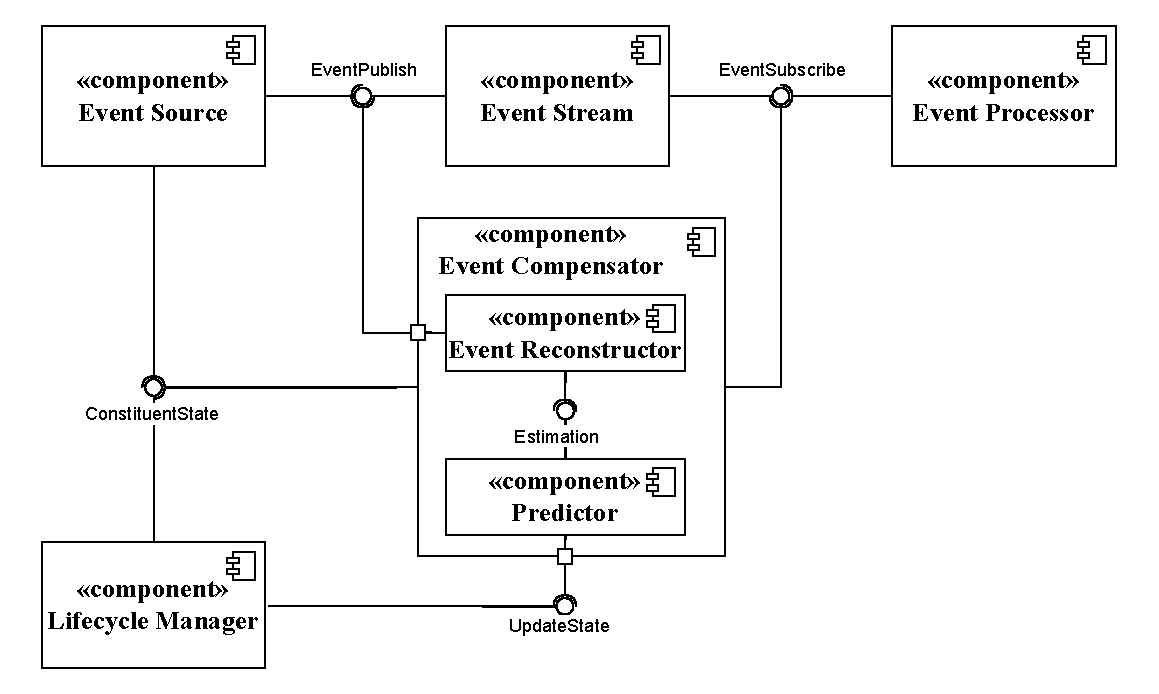
\includegraphics[width=0.65\textwidth]{figures/Architecture/High Level Component Diagram.drawio.pdf}
\caption{Component model of the demonstrated architecture}
\label{fig:component-model}
\end{figure}

As shown in \figref{fig:component-model}, constituent behaviour is coordinated by a \textbf{Lifecycle Manager} implemented using executable statecharts. \textbf{Event Sources} convert constituent observations into events and publish them to the \textbf{Event Stream}, where they are processed by an \textbf{Event Processor} to detect higher-level behaviours. When disturbances affect event availability, an \textbf{Event Compensator} reconstructs missing observations using predicted measurements.

The primary architectural components and their responsibilities are:

\begin{itemize}

\item \textbf{Lifecycle Manager} maintains the lifecycle state of each constituent using executable statecharts and exposes this state to other components.

\item \textbf{Event Source} converts measured observations into events and publishes them to the event stream according to the constituent's lifecycle state.

\item \textbf{Event Stream} distributes events between producers and consumers in the processing pipeline using a publish–subscribe model.

\item \textbf{Event Processor} consumes events from the stream and detects higher-level system behaviours through event pattern detection.

\item \textbf{Event Compensator} monitors the event stream and reconstructs missing observations when disturbances occur. It contains:
\begin{itemize}
\item \textbf{Event Reconstructor}, which publishes reconstructed events back into the stream.
\item \textbf{Predictor}, which estimates expected measurements used during reconstruction.
\end{itemize}

\end{itemize}



\section{System Implementation}
The architecture is implemented as an event-driven middleware composed of Python-based coordination services and a Java-based CEP processing engine. The Python middleware manages lifecycle state and event generation, with the \textit{lifecycle manager} implemented using executable statecharts developed with Itemis CREATE. Events are processed using an \textit{event processor} implemented with the Esper CEP engine. An \textit{event compensator} operates alongside the processing pipeline, monitoring the stream for missing observations and reconstructing events when disturbances occur using a \textit{predictor} implemented as a Kalman filter.
\section{UML Model of Implementation}

\begin{figure}[htp]
\centering
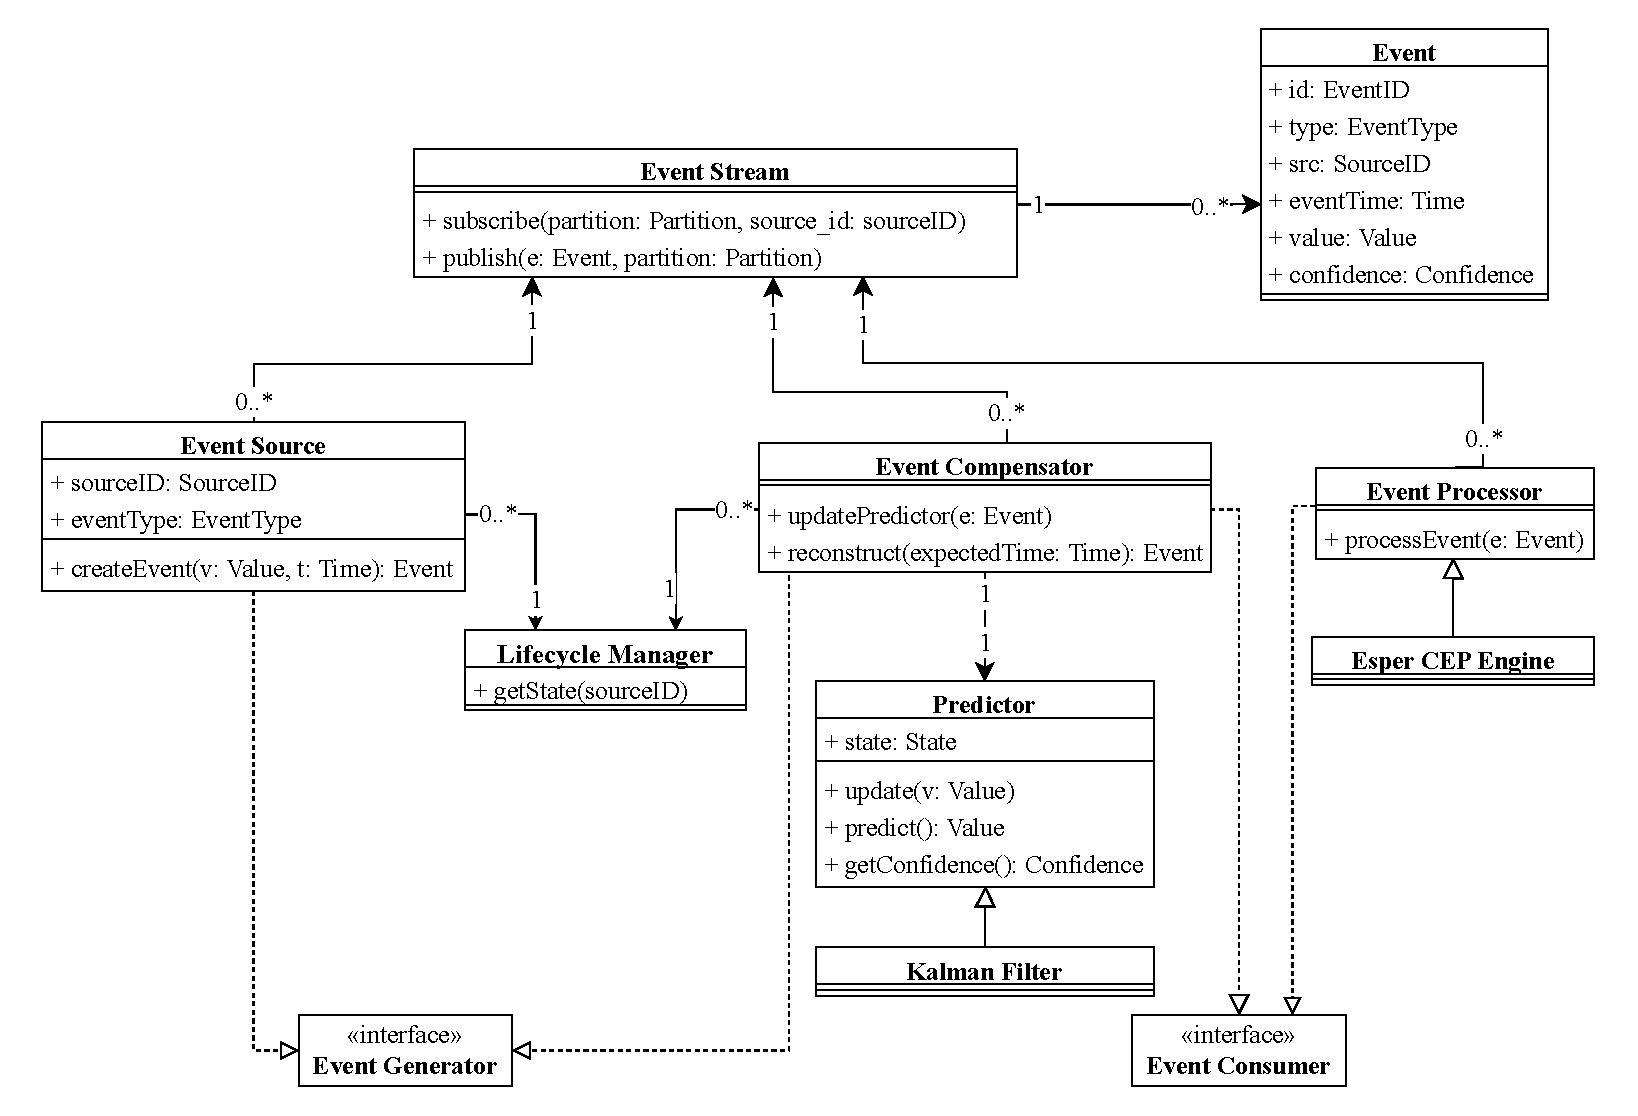
\includegraphics[width=0.9\textwidth]{figures/Architecture/UML Model.drawio.pdf}
\caption{UML model of architecture}
\label{fig:uml-model}
\end{figure}

Figure~\ref{fig:uml-model} illustrates how the architectural components are realized in the runtime system. The \textit{event stream} provides publish–subscribe communication between multiple producers and consumers. \textit{Event sources} publish events derived from constituent observations, while the \textit{lifecycle manager} exposes the state used to determine whether observations are emitted. The \textit{event compensator} monitors the stream and updates its \textit{predictor} as events arrive, consulting the lifecycle manager to determine when reconstruction is permitted. When disturbances occur, reconstructed events are published back into the stream. Event processing is performed by the \textit{event processor} using the Esper CEP engine, while the \textit{predictor} used for reconstruction is implemented as a Kalman filter.


% lets rename this but the main point of this section is to now explain how we lets the statecharts envforce the relaibility constraints in the system from the model wek developed, we need to ensure thats the main focus I think and less strongly on the event stuff
\subsection{Operationalizing the SoTS Reliability Model}

The reliability model introduced in \chref{ch:reliable-sots} defines lifecycle constraints governing the participation of constituents within a SoTS. In the implementation presented here, these constraints are operationalized through executable statecharts that regulate how constituents interact with the event processing pipeline. Each constituent is associated with an executable lifecycle controller that maintains the constituent's belonging and health state. These state machines determine when constituents emit observations and when compensation mechanisms are permitted to reconstruct missing data.

% Here should explain itemis create, code generation to create runtime interface that we can couple behaviours to
\subsubsection{Executable Lifecycle Statecharts}

Lifecycle statecharts are implemented using Itemis CREATE, which provides a modelling environment for defining state machines and generating executable code.

\begin{figure}[htp]
\centering
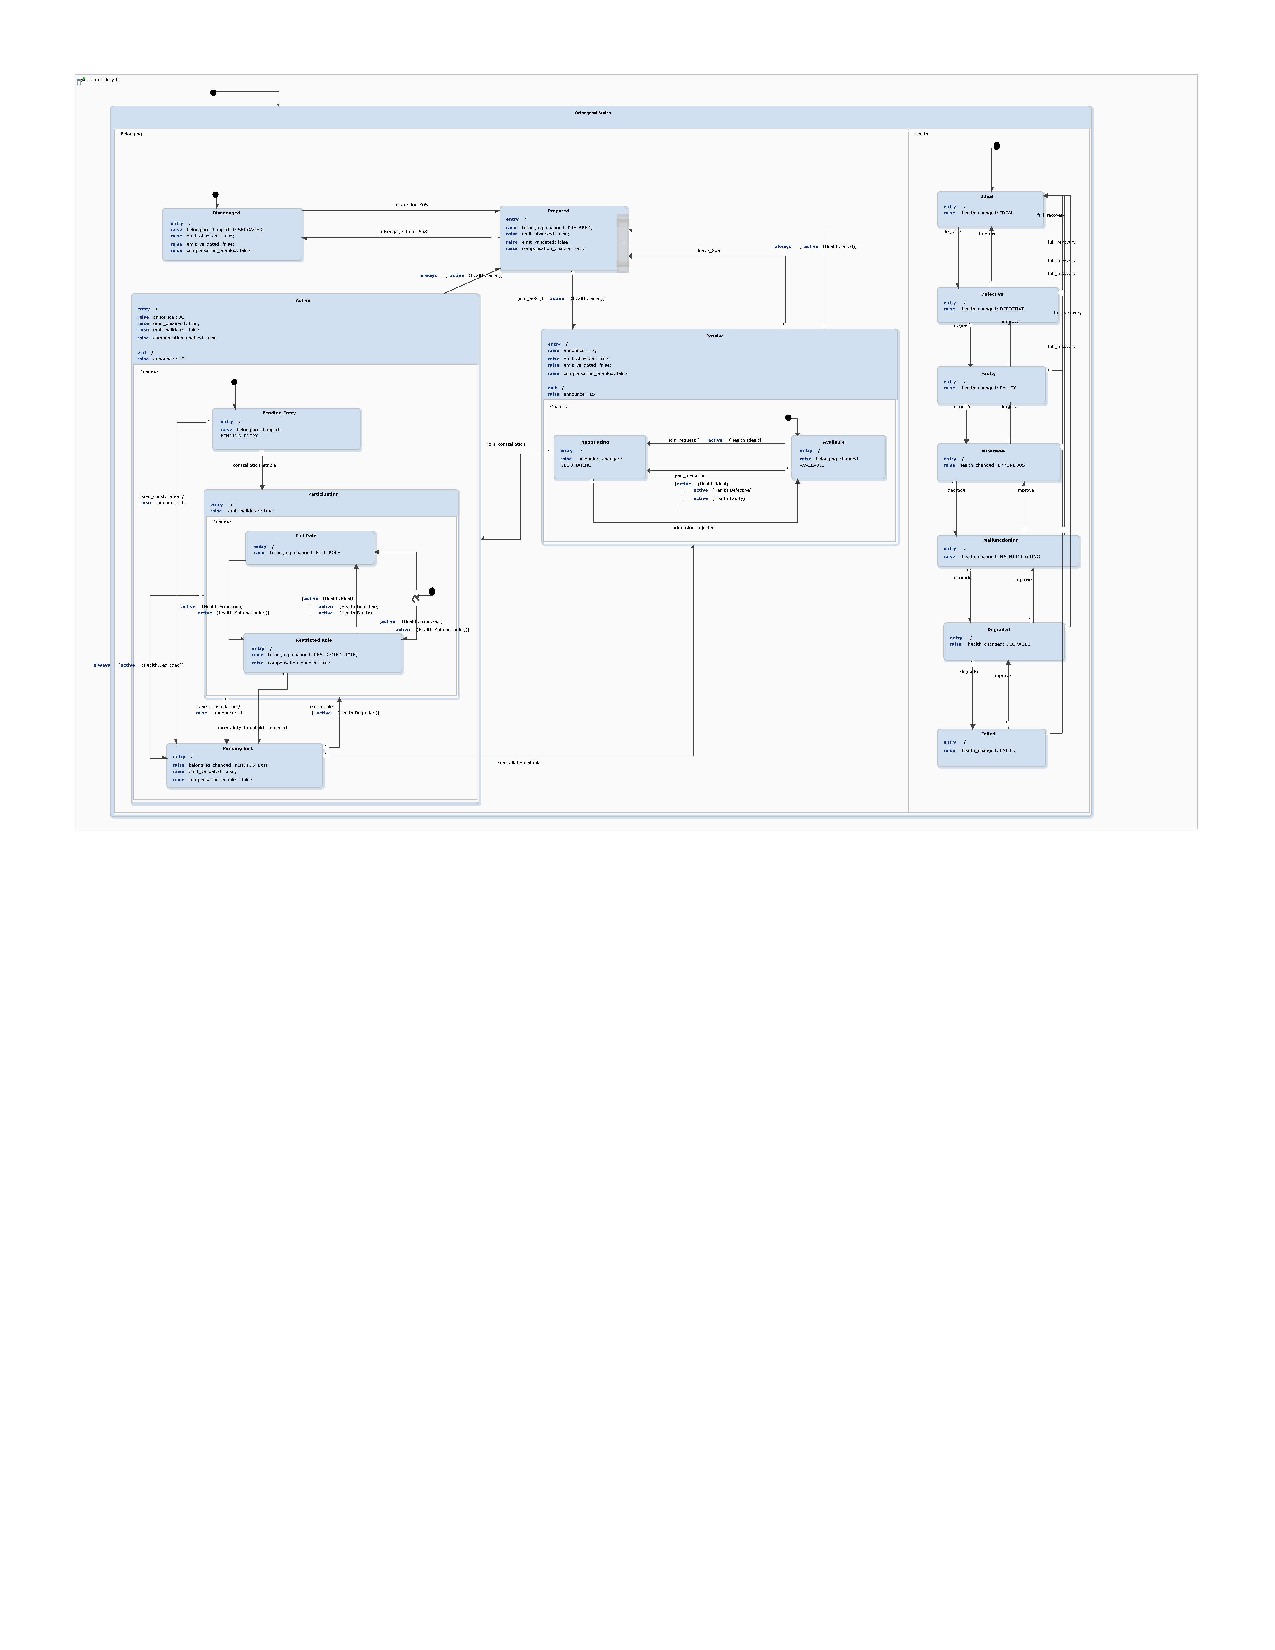
\includegraphics[width=0.7\textwidth]{figures/Architecture/itemis.pdf}
\caption{Level 4: Adaptive SoTS implemented in Itemis Create}
\label{fig:itemis-diagram}
\end{figure}

The Python code generator is used to compile the lifecycle models into executable controllers integrated with the runtime system. Each constituent is associated with a statechart instance that exposes lifecycle states, transitions, and events through a runtime interface. This allows system components to raise lifecycle events and query the current state during execution.


% Lets rename this to something more clear about what the section is supposed to be about, the entire point it to connect the theory we established to the actual runtime behaviour of the level 4
\subsubsection{State-Dependent Component Behaviour}

Lifecycle state determines how system components interact with the event processing pipeline. The statechart controller governs both the emission of observations and the activation of compensation mechanisms. Event sources consult the statechart controller before emitting observations, while the compensation service uses the same lifecycle state to determine when estimator updates and event reconstruction are permitted. Table~\ref{tab:state-behaviour} summarizes these behaviours.

\begin{table}[htp]
\small
\centering
\caption{Lifecycle state effects on events, compensation, and prediction}
\label{tab:state-behaviour}
\begin{tabular}{l c c c}
\toprule
\textbf{Lifecycle State} 
& \makecell{\textbf{Contributes} \\ \textbf{Events}} 
& \makecell{\textbf{Uses} \\ \textbf{Compensation}} 
& \makecell{\textbf{Updates} \\ \textbf{Predictor}} \\
\midrule


Disengaged &  &  &  \\
Prepared &  &  &  \\

\midrule
Passive (Negotiating) &  &  & $\checkmark$ \\
Passive (Available) &  &  & $\checkmark$ \\

\midrule
Active (Pending Entry) &  &  & $\checkmark$ \\
Active (Full Role) & $\checkmark$ &  & $\checkmark$ \\
Active (Restricted Role) & $\checkmark$ & $\checkmark$ & $\checkmark$ \\
Active (Pending Exit) &  &  & $\checkmark$ \\

\bottomrule
\end{tabular}
\end{table}

\textit{Event emission.} Constituents emit observations only when operating in the Full Role state, where events are forwarded to the CEP engine for processing. In all other states, event emission is suppressed, although observed events may still be used to update the state estimator. \textit{Event reconstruction.} When degradation causes a transition to the Restricted Role, observations may become incomplete. In this state, the compensation service reconstructs missing events to maintain a consistent event stream. \textit{Estimator updates.} The state estimator updates whenever observed events are available. Updates occur across passive and active states, allowing the system to maintain an internal estimate of system behaviour even when events are not forwarded to the CEP engine.


\subsection{Supporting Event Processing Infrastructure}
% explai9n an overview of the pipeline, in terms of the observations, turned to events, whcih are pushed to the stream and cep with an additional compensation mechanism
The event processing pipeline distributes observations between system components through a shared event stream. Observations produced by constituents are translated into events by Python-based middleware services and analysed by a Java-based CEP engine to derive system-level behaviour. These layers are connected through a language-independent messaging infrastructure.


% Then we need to go through all these subsubsections but condense them to what is necessary only to support our ideas about the state charts
\subsubsection{Event Generation from Constituent Observations}

Event sources act as the interface between observations produced by constituent systems and the event stream processed by the SoTS. Each event source is associated with a constituent DT and translates system observations into structured events containing attributes such as timestamp, constituent identifier, event type, and payload.

The publishing behaviour of an event source is controlled by the lifecycle state exposed by the statechart controller. Before emitting an event, the event source checks the current lifecycle state to determine whether observations should be suppressed, published for CEP processing, or used internally for services such as updating the state estimator.

Event sources therefore perform three primary responsibilities:

\begin{itemize}
\item translating system observations into events,
\item serializing event data into a standardized representation,
\item publishing events according to the lifecycle state of the constituent.
\end{itemize}


\subsubsection{Event Transport using ZeroMQ}

Event transport is implemented using ZeroMQ (ZMQ) \cite{zeromq_org}, which provides a lightweight publish--subscribe messaging model for asynchronous communication between system components. ZMQ serves as a cross-language messaging layer that connects Python-based middleware services with the Java-based CEP engine. Event sources, compensation services, and lifecycle controllers operate within the Python runtime, while the CEP engine executes within a separate Java environment. Events are serialized as JSON messages and published to the event stream, where a ZMQ broker routes messages from publishers to subscribed components. This messaging layer enables heterogeneous components implemented in different programming languages to exchange events through a common communication infrastructure while remaining loosely coupled.

\begin{table}[t]
\centering
\footnotesize
\caption{ZMQ topic structure and subscription patterns}
\label{tab:zmq-topics}
\begin{tabularx}{\textwidth}{p{4.5cm} X X}
\toprule
\textbf{Topic pattern} & \textbf{Event type} & \textbf{Example subscribers} \\
\midrule
\texttt{*} &
All events (observed and reconstructed) &
Event processor \\

\texttt{observed.<source\_id>} &
Observed events from a specific source &
Coordinator, Analytics components \\

\texttt{observed.*} &
Observed events from all sources &
Coordinator \\

\texttt{reconstructed.<source\_id>} &
Reconstructed events for a specific source &
Event processor, Visualization components \\
\bottomrule
\end{tabularx}
\end{table}


Topic-based routing is used to organize events within the messaging layer. Observed events are published under topics of the form \texttt{observed.<source\_id>}, while reconstructed events are published under \texttt{reconstructed.<source\_id>}. This allows downstream components to selectively subscribe to the events relevant to their responsibilities.



\subsubsection{Complex Event Processing with Esper}

Event analysis within the pipeline is performed using the Esper CEP engine \cite{esper_reference}. The CEP engine runs within a Java runtime and consumes events from the ZeroMQ event stream produced by the Python-based middleware. Events distributed through the stream are forwarded to Esper, where queries written in the Event Processing Language (EPL) detect higher-level behaviours from incoming observations.

\begin{lstlisting}[language=json, basicstyle=\footnotesize\ttfamily, caption={Example atomic event pattern definitions}, label={lst:atomic-patterns}]
[
  {
    "name": "Overspeeding",
    "type": "atomic",
    "epl": "@Name('Overspeeding') select e from Event as e where e.src='speed-1' and e.value > 25 and confidence > 0.75"
  }
]
\end{lstlisting}

The implementation distinguishes between \textit{atomic} and \textit{complex} event patterns. Atomic patterns define conditions over individual events based on attributes such as source identifiers, measurement values, and confidence levels. Complex patterns combine previously detected events to identify correlated behaviours across multiple constituents or time intervals. Through this pattern composition, the CEP engine derives system-level conditions that cannot be inferred from individual observations alone.




\subsection{Compensation for Disturbances in Event Streams}

In the Level~4 reliability configuration introduced in \chref{ch:reliable-sots}, constituents operating in restricted roles may produce reduced or degraded observations. To maintain reliable system-level reasoning under these conditions, the architecture includes a compensation service that supplements the event stream when constituent behaviour degrades. The compensation service operates as a middleware component that monitors the event stream and supplements observations when compensatory behaviour is required. The service maintains an internal estimate of system behaviour and uses this estimate to generate reconstructed events when appropriate. Reconstructed events are reinserted into the event stream, allowing downstream components such as the CEP engine to continue operating on a consistent stream of observations.

\subsubsection{State Estimation using Kalman Filtering}

State estimation within the compensation service is implemented using Kalman filters \cite{kalman1960filtering}. Each constituent is associated with an estimator that maintains an internal model of system behaviour and is updated whenever observations are available. When compensatory behaviour is required, the estimator generates predicted observations that are used to reconstruct events within the pipeline. In the implementation presented here, the estimators are implemented in Python using the FilterPy library \cite{labbe2014kalman}.

In addition to producing state estimates, the estimator provides a measure of prediction consistency based on the normalized innovation squared (NIS), a commonly used diagnostic for evaluating Kalman filter performance \cite{bar2001estimation,simon2006optimal}. NIS values are used to derive confidence scores associated with reconstructed events, which are attached to events before they are reintroduced into the event stream.



\subsection{Processing Workflow}
The previous sections described the architectural components responsible for lifecycle control, event generation, event streaming, and compensation. Figure~\ref{fig:event-sequence} illustrates how these components interact during runtime.

\begin{figure}[t]
\centering
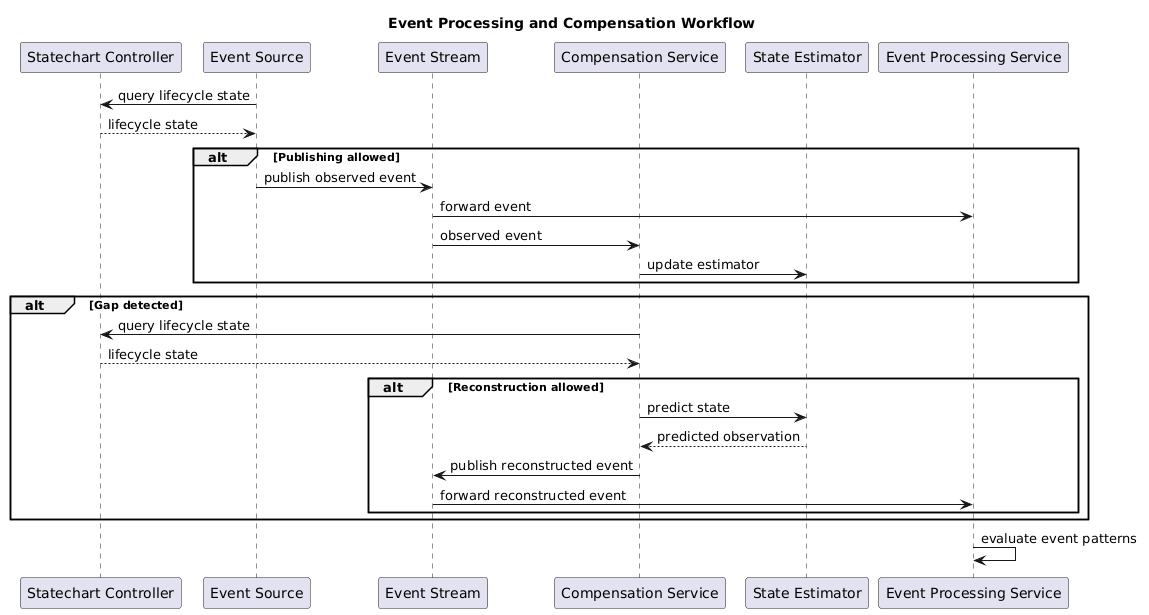
\includegraphics[width=\textwidth]{figures/Architecture/Sequence Diagram.png}
\caption{Sequence diagram}
\label{fig:event-sequence}
\end{figure}

In this workflow, the event source consults the statechart controller before publishing observations to the event stream. The compensation service monitors the stream to update the state estimator and detect gaps in event generation. When permitted by the lifecycle state, reconstructed events are generated and reintroduced into the event stream for downstream processing by the event processing service.




\section{Evaluation Setup and Disturbance Injection}

% To evaluate system behaviour under degraded conditions, the implementation includes a disturbance injector that modifies the behaviour of event sources during execution. Disturbances are defined through configuration files that specify event dropouts and lifecycle transitions affecting constituent participation. Scenarios are generated using deterministic random seeds so that identical disturbance patterns can be reproduced across experimental runs.

% Each scenario is executed under three experimental configurations:

% \begin{enumerate}
% \item \textbf{Oracle}: Ground truth execution without disturbances, providing a reference event stream.
% \item \item \textbf{Compensation}: Disturbances are applied while Kalman-based event reconstruction is enabled.
% \item \textbf{No Compensation}: Disturbances are applied while compensation mechanisms are disabled.

% \end{enumerate}

% Disturbances are introduced by modifying the behaviour of DT event sources based on their health state. As health degrades, the likelihood of event dropouts increases while the probability of recovery decreases. These parameters are defined in the disturbance configuration and summarized in Table~\ref{tab:disturbance-config}.

% \begin{table}[h]
% \centering
% \caption{Disturbance configuration by constituent health level}
% \label{tab:disturbance-config}
% \begin{tabular}{lccc}
% \toprule
% \textbf{Health Level} & \textbf{Dropout Probability} & \textbf{Recovery Probability} & \textbf{Lifecycle Behaviour} \\
% \midrule
% Ideal & 0.00 & 0.00 & Full participation \\

% Defective & 0.05 & 0.30 & Temporary degradation possible; typically remains active \\

% Faulty & 0.15 & 0.20 & May transition to restricted role; intermittent recovery possible \\

% Erroneous & 0.30 & 0.10 & Restricted participation likely; occasional exit and rejoin \\

% Malfunctioning & 0.50 & 0.05 & Frequent restricted participation; temporary exit possible \\

% Degraded & 0.70 & 0.02 & High likelihood of exit from active participation \\

% Failed & 1.00 & 0.00 & Forced exit from participation \\

% \bottomrule
% \end{tabular}
% \end{table}

% During execution, the system records metrics describing the resulting event streams and pattern detection behaviour. These include counts of observed and reconstructed events, detection outcomes for CEP patterns, and confidence values associated with reconstructed observations. These metrics are analyzed in the following chapter to evaluate the effectiveness of the proposed reliability mechanisms.











